

\tikzset{every picture/.style={line width=0.75pt}} %set default line width to 0.75pt        

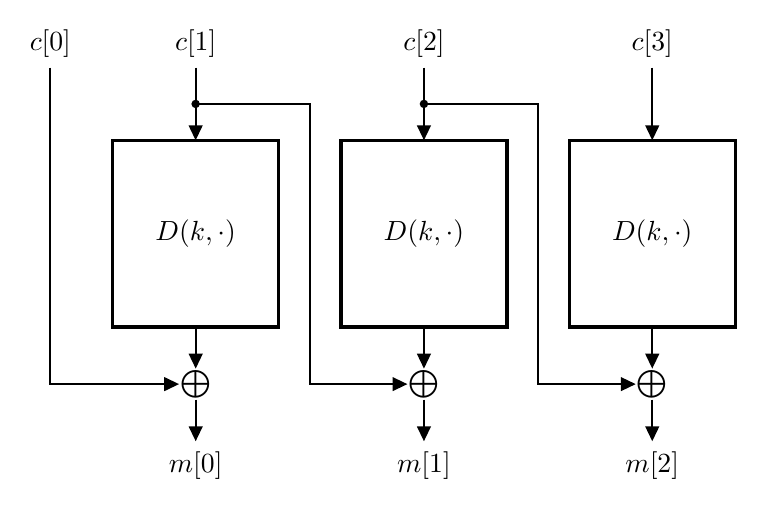
\begin{tikzpicture}[x=0.75pt,y=0.75pt,yscale=-1,xscale=1]
%uncomment if require: \path (0,263); %set diagram left start at 0, and has height of 263

%Shape: Rectangle [id:dp5106849726463678] 
\draw  [line width=1.2]  (90,80) -- (170,80) -- (170,170) -- (90,170) -- cycle ;
%Straight Lines [id:da17601265821305034] 
\draw    (130,45) -- (130,77) ;
\draw [shift={(130,80)}, rotate = 270] [fill={rgb, 255:red, 0; green, 0; blue, 0 }  ][line width=0.08]  [draw opacity=0] (7.14,-3.43) -- (0,0) -- (7.14,3.43) -- cycle    ;
%Straight Lines [id:da5432224444295874] 
\draw    (130.03,170) -- (130.03,187) ;
\draw [shift={(130.03,190)}, rotate = 270] [fill={rgb, 255:red, 0; green, 0; blue, 0 }  ][line width=0.08]  [draw opacity=0] (7.14,-3.43) -- (0,0) -- (7.14,3.43) -- cycle    ;
%Shape: Rectangle [id:dp7814760720667226] 
\draw  [line width=1.2]  (200,80) -- (280,80) -- (280,170) -- (200,170) -- cycle ;
%Straight Lines [id:da8079846565492814] 
\draw    (240,45) -- (240,77) ;
\draw [shift={(240,80)}, rotate = 270] [fill={rgb, 255:red, 0; green, 0; blue, 0 }  ][line width=0.08]  [draw opacity=0] (7.14,-3.43) -- (0,0) -- (7.14,3.43) -- cycle    ;
%Shape: Rectangle [id:dp012526395676392799] 
\draw  [line width=1.2]  (310,80) -- (390,80) -- (390,170) -- (310,170) -- cycle ;
%Straight Lines [id:da33169300529204415] 
\draw    (350,45) -- (350,77) ;
\draw [shift={(350,80)}, rotate = 270] [fill={rgb, 255:red, 0; green, 0; blue, 0 }  ][line width=0.08]  [draw opacity=0] (7.14,-3.43) -- (0,0) -- (7.14,3.43) -- cycle    ;
%Straight Lines [id:da04062621189844484] 
\draw    (130.03,205) -- (130.03,222) ;
\draw [shift={(130.03,225)}, rotate = 270] [fill={rgb, 255:red, 0; green, 0; blue, 0 }  ][line width=0.08]  [draw opacity=0] (7.14,-3.43) -- (0,0) -- (7.14,3.43) -- cycle    ;
%Straight Lines [id:da25574292241048324] 
\draw    (240,170) -- (240,187) ;
\draw [shift={(240,190)}, rotate = 270] [fill={rgb, 255:red, 0; green, 0; blue, 0 }  ][line width=0.08]  [draw opacity=0] (7.14,-3.43) -- (0,0) -- (7.14,3.43) -- cycle    ;
%Straight Lines [id:da09615282132922487] 
\draw    (240,205) -- (240,222) ;
\draw [shift={(240,225)}, rotate = 270] [fill={rgb, 255:red, 0; green, 0; blue, 0 }  ][line width=0.08]  [draw opacity=0] (7.14,-3.43) -- (0,0) -- (7.14,3.43) -- cycle    ;
%Straight Lines [id:da7942138401350809] 
\draw    (350,170) -- (350,187) ;
\draw [shift={(350,190)}, rotate = 270] [fill={rgb, 255:red, 0; green, 0; blue, 0 }  ][line width=0.08]  [draw opacity=0] (7.14,-3.43) -- (0,0) -- (7.14,3.43) -- cycle    ;
%Straight Lines [id:da8121225965074672] 
\draw    (350,205) -- (350,222) ;
\draw [shift={(350,225)}, rotate = 270] [fill={rgb, 255:red, 0; green, 0; blue, 0 }  ][line width=0.08]  [draw opacity=0] (7.14,-3.43) -- (0,0) -- (7.14,3.43) -- cycle    ;
%Straight Lines [id:da23227714375359465] 
\draw    (60,45) -- (60,197.5) -- (119,197.5) ;
\draw [shift={(122,197.5)}, rotate = 180] [fill={rgb, 255:red, 0; green, 0; blue, 0 }  ][line width=0.08]  [draw opacity=0] (7.14,-3.43) -- (0,0) -- (7.14,3.43) -- cycle    ;
%Straight Lines [id:da34741017759169557] 
\draw    (130,62.5) -- (185,62.5) -- (185,197.5) -- (229,197.5) ;
\draw [shift={(232,197.5)}, rotate = 180] [fill={rgb, 255:red, 0; green, 0; blue, 0 }  ][line width=0.08]  [draw opacity=0] (7.14,-3.43) -- (0,0) -- (7.14,3.43) -- cycle    ;
%Straight Lines [id:da05014436659836896] 
\draw    (240,62.5) -- (295,62.5) -- (295,197.5) -- (339,197.5) ;
\draw [shift={(342,197.5)}, rotate = 180] [fill={rgb, 255:red, 0; green, 0; blue, 0 }  ][line width=0.08]  [draw opacity=0] (7.14,-3.43) -- (0,0) -- (7.14,3.43) -- cycle    ;
%Shape: Circle [id:dp973486631127561] 
\draw  [fill={rgb, 255:red, 0; green, 0; blue, 0 }  ,fill opacity=1 ] (128.5,62.5) .. controls (128.5,61.67) and (129.17,61) .. (130,61) .. controls (130.83,61) and (131.5,61.67) .. (131.5,62.5) .. controls (131.5,63.33) and (130.83,64) .. (130,64) .. controls (129.17,64) and (128.5,63.33) .. (128.5,62.5) -- cycle ;
%Shape: Circle [id:dp31728957795364554] 
\draw  [fill={rgb, 255:red, 0; green, 0; blue, 0 }  ,fill opacity=1 ] (238.5,62.5) .. controls (238.5,61.67) and (239.17,61) .. (240,61) .. controls (240.83,61) and (241.5,61.67) .. (241.5,62.5) .. controls (241.5,63.33) and (240.83,64) .. (240,64) .. controls (239.17,64) and (238.5,63.33) .. (238.5,62.5) -- cycle ;

% Text Node
\draw (130,125) node    {$D( k,\cdot )$};
% Text Node
\draw (60,41.6) node [anchor=south] [inner sep=0.75pt]    {$c[ 0]$};
% Text Node
\draw (130.03,228.4) node [anchor=north] [inner sep=0.75pt]    {$m[ 0]$};
% Text Node
\draw (240,125) node    {$D( k,\cdot )$};
% Text Node
\draw (130,41.6) node [anchor=south] [inner sep=0.75pt]    {$c[ 1]$};
% Text Node
\draw (240,228.4) node [anchor=north] [inner sep=0.75pt]    {$m[ 1]$};
% Text Node
\draw (350,125) node    {$D( k,\cdot )$};
% Text Node
\draw (240,41.6) node [anchor=south] [inner sep=0.75pt]    {$c[ 2]$};
% Text Node
\draw (350,228.4) node [anchor=north] [inner sep=0.75pt]    {$m[ 2]$};
% Text Node
\draw (130,197.5) node    {$\bigoplus $};
% Text Node
\draw (240,197.5) node    {$\bigoplus $};
% Text Node
\draw (350,197.5) node    {$\bigoplus $};
% Text Node
\draw (350,41.6) node [anchor=south] [inner sep=0.75pt]    {$c[ 3]$};


\end{tikzpicture}